\documentclass[conference]{IEEEtran}

\ifCLASSOPTIONcompsoc
  % IEEE Computer Society needs nocompress option
  % requires cite.sty v4.0 or later (November 2003)
  \usepackage[nocompress]{cite}
\else
  % normal IEEE
  \usepackage{cite}
\fi

% All pdf figures are stored in this folder
\usepackage[pdftex]{graphicx}
\usepackage[T1]{fontenc}
\usepackage{array}
\graphicspath{{./figures/}}

\newcommand\uml[1]{\texttt{\textbf{#1}}}
\newcommand\cg[1]{\textit{#1}}
\usepackage{xcolor,colortbl}
\definecolor{Gray}{gray}{0.85}
% *** GRAPHICS RELATED PACKAGES ***
%
\ifCLASSINFOpdf
  % \usepackage[pdftex]{graphicx}
  % declare the path(s) where your graphic files are
  % \graphicspath{{../pdf/}{../jpeg/}}
  % and their extensions so you won't have to specify these with
  % every instance of \includegraphics
  % \DeclareGraphicsExtensions{.pdf,.jpeg,.png}
\else
  % or other class option (dvipsone, dvipdf, if not using dvips). graphicx
  % will default to the driver specified in the system graphics.cfg if no
  % driver is specified.
  % \usepackage[dvips]{graphicx}
  % declare the path(s) where your graphic files are
  % \graphicspath{{../eps/}}
  % and their extensions so you won't have to specify these with
  % every instance of \includegraphics
  % \DeclareGraphicsExtensions{.eps}
\fi

\hyphenation{op-tical net-works semi-conduc-tor}

\begin{document}
%
% paper title
% Titles are generally capitalized except for words such as a, an, and, as,
% at, but, by, for, in, nor, of, on, or, the, to and up, which are usually
% not capitalized unless they are the first or last word of the title.
% Linebreaks \\ can be used within to get better formatting as desired.
% Do not put math or special symbols in the title.
\title{When Asteroids Attack: The MWSU Simulation Team's Adventure in High Level Architecture and Distributed Simulation}
% author names and affiliations
% use a multiple column layout for up to three different
% affiliations

% conference papers do not typically use \thanks and this command
% is locked out in conference mode. If really needed, such as for
% the acknowledgment of grants, issue a \IEEEoverridecommandlockouts
% after \documentclass

% for over three affiliations, or if they all won't fit within the width
% of the page (and note that there is less available width in this regard for
% compsoc conferences compared to traditional conferences), use this
% alternative format:
%

\author{\IEEEauthorblockN{Bingyang Wei\IEEEauthorrefmark{1},
Amy Knowles, Chris Silva, Christine Mounce}
\IEEEauthorblockA{Department of Computer Science\\
Midwestern State University,
Wichita Falls, Texas 76308\\ \IEEEauthorrefmark{1}Email: bingyang.wei@mwsu.edu}}

% make the title area
\maketitle

% As a general rule, do not put math, special symbols or citations
% in the abstract
\begin{abstract}
The Simulation Exploration Experience (SEE) is an annual, inter-university, distributed simulation challenge led by NASA. A primary objective is to provide a platform for college students to work in highly dispersed teams to design, develop, test, and execute a simulated lunar mission using High Level Architecture. During the SEE in 2016, 19 federates developed by student teams from three continents successfully joined the HLA federation and collaborated to accomplish a lunar mission. The Midwestern State University team first participated in SEE 2016 by developing a communication satellite federate which broadcast an alert about the incoming of an asteroid to physical entities on the surface of the moon. This paper describes SEE, High Level Architecture, the MWSU Sim Team experience, lessons learned and recommendations for future teams.
\end{abstract}

% For peer review papers, you can put extra information on the cover
% page as needed:
% \ifCLASSOPTIONpeerreview
% \begin{center} \bfseries EDICS Category: 3-BBND \end{center}
% \fi
%
% For peerreview papers, this IEEEtran command inserts a page break and
% creates the second title. It will be ignored for other modes.
\IEEEpeerreviewmaketitle

\section{Introduction}
Initiated in 2011, the annual Simulation Exploration Experience event, formally known as SISO Smackdown, has successfully promoted the awareness of the use of High Level Architecture (HLA) in distributed simulation around the world. During the event, academia, industry and professional associations collaborate to design, develop, test and demonstrate a simulated lunar mission. SEE provides an excellent platform for college students to learn and practice both M\&S and software engineering concepts and principles. More importantly, the opportunity of working closely with M\&S professionals in industry and associations is an invaluable experience to the students. 

During SEE 2016, a lunar mission was simulated. NASA Johnson Space Center (JSC), Kennedy Space Center (KSC) and 12 universities from three continents participated in this year\rq{}s distributed simulation event. All participants conformed to the IEEE HLA standard 1516-2010 for modeling and simulation. As usual, NASA provided basic support to the entire simulation mission, JSC regulated the time of the simulation while KSC provided real-time visualization of the simulation mission. Each university contributed to the lunar simulation by implementing a part of the entire simulation called a federate (More HLA terminologies are available in \cite{HLA}). A description of the SEE 2016 simulated mission follows: Astronauts explore a huge impact crater close to the south pole of the moon, called Aitken Basin.  Viewers are then introduced to a number of new lunar research units and construction sites: a 3D-printing site by University of Alberta (Canada), a supply depot, oxidizer and propellant production facility by University of Bordeaux (France), an astronaut habitat site by Facens (Brazil), a cargo rover by Florida Institute of Technology, a fuel rover by University of Nebraska, a lunar buggy and an unmanned aerial vehicle (UAV) by University of Liverpool (England).

The peaceful exploration operation is suddenly interrupted by the detection of an incoming asteroid by an asteroid detection system developed by University of Genoa (Italy). The command and communication center \cite{falcone2014simulation} developed by University of Calabria (Italy) alerts all physical entities on the surface of the moon, and the communication satellites developed by Midwestern State University alert the lunar buggy which is out of reach of the command and control center.

During the simulation, all federates were connected successfully to the runtime infrastructure (RTI) provided by Pitch Technologies and advancing time (see Figure \ref{Federation}). Each rectangle represents a joined federate and the middle gray bar denotes the RTI.
\begin{figure}[!htbp]
	\centering
		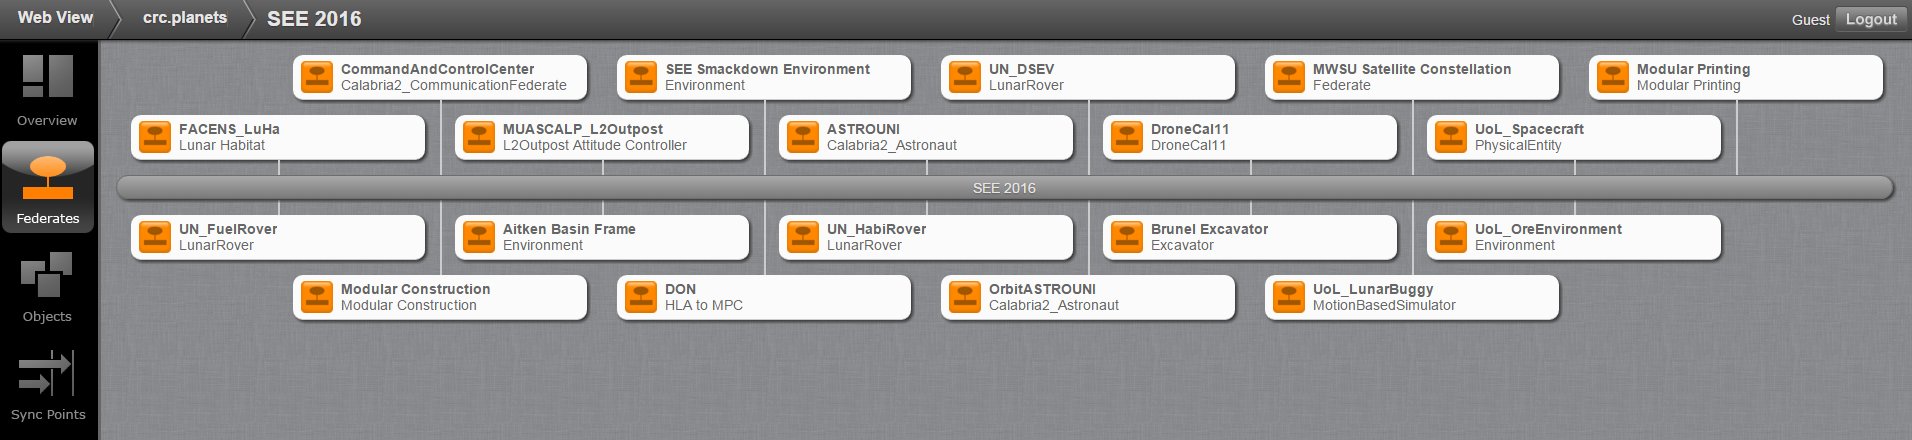
\includegraphics[width=\linewidth]{Pitch.PNG}
		\caption{Federates connecting through Pitch RTI.}
	\label{Federation}
\end{figure}

This paper concentrates on the learning experience of Midwestern State University team members, their interactions with other student teams across the world, industry representatives from Pitch, and NASA engineers at both JSC and KSC.  The rest of the paper is structured as follows: Section II provides an introduction to High Level Architecture (HLA); Section III describes in detail the 2016 experience of the Midwestern State University (MWSU) team; Lessons learned from SEE is discussed in Section IV and Section VI concludes the paper and provides instructions for future teams to join SEE.

\section{High Level Architecture}

\section{2016 SEE Experience}

\section{Lessons Learned}
During the integration test and the final demo, we found several problems with our federate.  The MWSU federate was able to locate all physical entities in the Insight3D viewer, and verify the location and motion information of different entities in the orbit of the moon or on the surface.  

However, several problems with our federate were found during the integration testing:

Problem 1: Significant time required to populate six satellites.
Solution: This problem is understandable, as the STK numerical propagator calculates a large amount of data for each satellite in order to achieve high fidelity rendering.  By using background calculation capabilities, we achieved a reduction in the time required by parallelizing the satellite propagations.

Problem 2: MWSU federate worked well with Pitch RTI but failed to run on M{\"A}K RTI. When testing on M{\"A}K RTI, exception ``unsatisfiedLinkError makRtiJava1516e.dll: the specified procedure could not be found\rq\rq{} is thrown.
Solution: MWSU federate is a Java application built in Eclipse. This is an old problem with M{\"A}K RTI which does not work with the most recent version of the Java IDE. We attempted to downgrade our Java IDE environment/code in order to communicate with the M{\"A}K RTI, as suggested by members of the 2012 UAHuntsville team \cite{bulgatz2012design}. We were unable to solve this problem and have informed engineers at VT M{\"A}K. We hope this issue can be fixed for SEE 2017.

Problem 3: MWSU federate kept throwing NullPointer exceptions due to other teams failing to provide the latest Attribute Handle Value Map or they provided Attribute Handle Value Map that misses certain attribute values.
Solution: It is a good software engineering principle to not expect federates developed by other teams to behave exactly as expected. Proper and robust exception handling mechanisms were added to help solve this problem.

Problem 4: For our Insight3D viewer, entities on the surface of the moon and those orbiting the moon were represented through markers and text. Since there were so many entities in 2016, the text and markers tended to bloat the viewer and hinder its readability.
Solution: A distance constraint on the visibility of the marker was added so that a marker would only become visible when the distance between the camera and the entity was less than 1000km. If the moon was viewed at a great distance, only the text representing the name of the entity could be seen in the Insight3D viewer.

Problem 5: During testing, we found that some HLA callbacks were never called when they were supposed to be called.
Solution: HLA provides different versions of the same callback, for instance, there are three reflectAttributeValues callbacks. Since the specific callback version the RTI would invoke could not be predicted with optimal success, we added all three callback versions defined in \uml{TheFederate} class and placed the same implementation code in three reflectAttributeValues() functions with different signatures.
 
Problem 6: When a federate resigned from the federation, the Insight3D viewer still kept the marker and text representing the physical entity of that resigned federate.
Solution: Added code to clear the marker and text when the callback method removeObjectInstance was called.

Problem 7: Synchronization exception occurred during the demonstration in insight3DTimeChanged() method of class \uml{LCANSatManager} due to different threads competing on the otherEntitiesToBeDrawn list. This caused the Insight3D viewer to crash.
Solution: Our current solution, although not optimal due to time constraints, was to surround the trouble code with a try-catch block in order to prevent the entire Insight3D viewer from crashing during the event. A better solution would be to add a mutual exclusion lock on this resource. The future team should be aware that this problem has not been solved properly.

\section{Conclusion}

% conference papers do not normally have an appendix

% trigger a \newpage just before the given reference
% number - used to balance the columns on the last page
% adjust value as needed - may need to be readjusted if
% the document is modified later
%\IEEEtriggeratref{8}
% The "triggered" command can be changed if desired:
%\IEEEtriggercmd{\enlargethispage{-5in}}

% references section

% can use a bibliography generated by BibTeX as a .bbl file
% BibTeX documentation can be easily obtained at:
% http://www.ctan.org/tex-archive/biblio/bibtex/contrib/doc/
% The IEEEtran BibTeX style support page is at:
% http://www.michaelshell.org/tex/ieeetran/bibtex/
\bibliographystyle{IEEEtran}
\bibliography{bibliography}
% argument is your BibTeX string definitions and bibliography database(s)
%\bibliography{IEEEabrv,../bib/paper}
%
% <OR> manually copy in the resultant .bbl file
% set second argument of \begin to the number of references
% (used to reserve space for the reference number labels box)

%\begin{thebibliography}{1}

%\bibitem{IEEEhowto:kopka}
%H.~Kopka and P.~W. Daly, \emph{A Guide to \LaTeX}, 3rd~ed.\hskip 1em plus
%  0.5em minus 0.4em\relax Harlow, England: Addison-Wesley, 1999.

%\end{thebibliography}




% that's all folks
\end{document}
